\newcommand{\figuraEnvolventeSolar}{%
\begin{figure}[H]
    \centering
    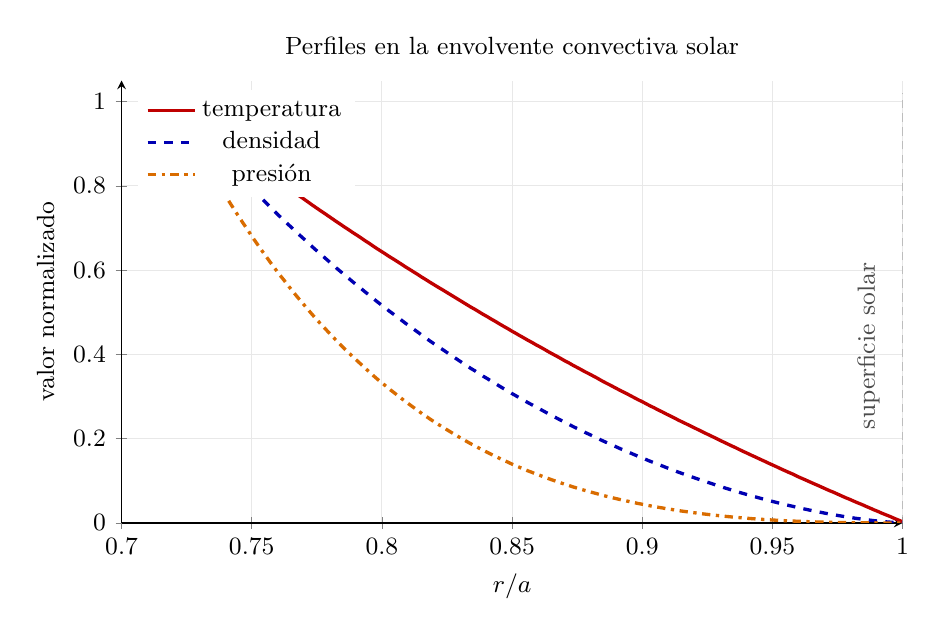
\begin{tikzpicture}[font=\small]
        \begin{axis}[
            width=11.5cm,
            height=7.2cm,
            xmin=0.70,xmax=1.00,
            ymin=0,ymax=1.05,
            axis lines=left,
            xlabel={$r/a$},
            ylabel={valor normalizado},
            title={Perfiles en la envolvente convectiva solar},
            grid=major,
            grid style={gray!18},
            samples=180,
            legend style={draw=none,fill=white,at={(0.02,0.98)},anchor=north west}]

            \addplot[very thick,red!75!black,domain=0.72:1]
                {(0.00111+1/x-1)/(0.00111+1/0.72-1)};
            \addlegendentry{temperatura}

            \addplot[very thick,blue!70!black,dashed,domain=0.72:1]
                {((0.00111+1/x-1)/(0.00111+1/0.72-1))^1.5};
            \addlegendentry{densidad}

            \addplot[very thick,orange!85!black,dash dot,domain=0.72:1]
                {((0.00111+1/x-1)/(0.00111+1/0.72-1))^2.5};
            \addlegendentry{presión}

            \draw[densely dashed,gray!70]
                (axis cs:1,0)--(axis cs:1,1.02);
            \node[rotate=90,anchor=south,text=black!70]
                at (axis cs:0.995,0.42) {superficie solar};
        \end{axis}
    \end{tikzpicture}
    \caption{Perfiles normalizados de temperatura, densidad y presión para
    una envolvente convectiva con $\gamma=5/3$. Las tres cantidades decrecen
    hacia la superficie, y la presión presenta la caída más pronunciada.}
    \label{fig:envolvente-solar}
\end{figure}%
}